% Chapter Template

\chapter{M\'etodos} % Main chapter title

\label{Chapter3} % Change X to a consecutive number; for referencing this chapter elsewhere, use \ref{ChapterX}

%----------------------------------------------------------------------------------------
%	SECTION 1
%----------------------------------------------------------------------------------------
\paragraph{}
En este capitulo procederemos a explicitar los métodos utilizados para las diferentes etapas que se realizaron para este trabajo final. En principio vamos a encontrarnos con una descripción general de los m\'etodos propuestos para las etapas de preprocesamiento, extracci\'on de indicadores, segmentaci\'on, etc. En la misma secci\'on comentaremos acerca del entrenamiento y la clasificaci\'on de los indicadores.
\paragraph{}
En la secci\'on siguiente profundizaremos en la etapa de preprocesamiento analizando las dificultades que se esperan superar con la misma, las t\'ecnicas que se utilizaron tanto para remover el ruido como para mejorar el contraste una vez removido, y por \'ultimo una descripci\'on del pipeline utilizado.
\paragraph{}
Las \'ultimas dos secciones estar\'an dedicadas a la extracci\'on de indicadores de las im\'agenes procesadas y el entrenamiento de clasificadores para su clasificaci\'on, valga la redundancia.


\section{Descripci\'on general}

\paragraph{}
METODO SEGMENTACION

\paragraph{}
Como primera etapa del proceso para lograr segmentar los vasos de la retina se encuentra el preprocesamiento, el mismo esta destinado a remover de la imagen lo que se considera ruido y realzar el contraste de los vasos sangu\'ineos con el resto de la misma.\\
Las im\'agenes con fluoresc\'ina carecen de ruido generado por cuestiones \'opticas del m\'etodo de captura, como por ejemplo el color, pero no est\'an exentas del ruido generado por la cantidad de vasos que se encuentran por debajo de la retina en la coroide, dado que por la naturaleza del m\'etodo de captura estos peque\~nos vasos emiten luz en la frecuencia que el equipo recibe aunque en menor cantidad.

\paragraph{}
EXTRACCION DE INDICADORES

\paragraph{}
CLASIFICADORES

\paragraph{}
DIFERENCIAS ENTRE TIEMPO DE ENRTENAMIENTO, VALIDACION Y TEST


\section{Preprocesamiento}
\subsection{¿Por qu\'e?}
Al analizar los diferentes m\'etodos de captura de la retina podemos observar que en cada una de ellos, aunque en diferentes formas, existe ruido generado por la misma tecnolog\'ia de captura. Para obtener un resultado \'optimo debemos ser capaces de llevar el ruido mencionado al nivel m\'inimo. Para lograrlo se utilizan distintos algoritmos de preprocesamiento, cada uno de ellos mas o menos eficiente dependiendo del tipo de ruido que exista en la im\'agen.
\paragraph{}
Las im\'agenes de angiograf\'ia fluorescente fueron diseñadas espec\'ificamente para evitar el ruido generado generalmente por los efectos \'opticos de los m\'etodos de captura tradicionales por lo que encontramos que poseen un nivel de ruido muy por debajo del que podemos ver en las im\'agenes de fondo de ojo, pero por otro lado, al estar ideado para visualizar la circulaci\'on de la sangre muchas veces encontramos reflejadas en las im\'agenes estrucuturas venosas o arteriales que no son de inter\'es para el estudio realizado. Estas \'ultimas tambi\'en pueden considerarse ruido.
\paragraph{}
Como objetivos principales del preprocesamiento podemos destacar:
\begin{description}
  \item[Reducci\'on de ruido:] Eliminaci\'on de diferencias de intensidad que son generados por ruido producido generalmente por los elementos de captura de la im\'agen.
  \item[Realce de bordes:] Realzar los bordes para luego facilitar la detecci\'on de los mismos en la etapa de segmentaci\'on.
  \item[Suavizado de im\'agenes:] Permite normalizar las intensidades de los p\'ixeles que estan fuera de la \"normalidad\" del vecindario donde se encuentra.
\end{description}

\subsection{Algoritmos investigados}

Luego de realizar un an\'alisis de investigaci\'on acerca de los algoritmos de preprocesamiento existentes encontramos que aquellos que mejor se adaptaban a las necesidades de nuestra casu\'istica eran aquellos que respetaban los bordes al suavizar la im\'agen.
\paragraph{}
Por un lado analizamos los algoritmos mas adecuados para la eliminaci\'on del fondo de la im\'agen, para este fin decidimos analizar tanto la mediana como la media. Por el otro, buscamos algoritmos para la reducci\'on de ruido para im\'agenes de angiodraf\'ia fluorescente y decidimos quedarnos con el algoritomo de difusi\'on anisotr\'opica y el filtro de coherencia.

\subsubsection{Remoci\'on fondo}

Para la remoci\'on de fondo se utilizaron dos filtros diferentes, por un lado el filtro de media y por el otro un filtro de mediana. Tanto la media como la mediana son filtros de paso bajo, es decir, un filtro que aten\'ua las intensidades altas y mantienen las intensidades bajas. Este tipo de filtros intentan reducir el ruido suavizando. En nuestro caso, al ser utilizado con grandes ventanas, nos permiten obtener una imagen homogénea que podemos restar a la imagen original para remover el fondo.

\begin{figure}[H]
	\centering
  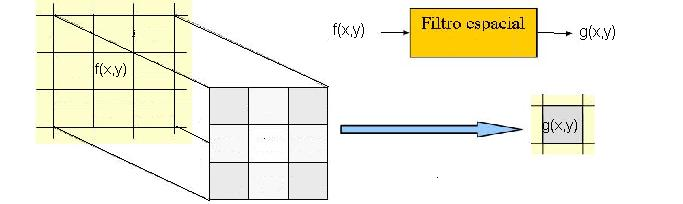
\includegraphics[width=0.75\textwidth]{./Figures/kernel.jpg}
  \caption{Filtros de convoluci\'on, se aplica sobre una ventana de nxn de vecinos al pixel que se analiza.}
  \label{fig:centeredregionthermal}
\end{figure}

\begin{description}
  \item[Media:] La media, como su nombre lo indica, realiza un promedio entre las instensidades vecinas al p\'ixel llevando a cabo una convoluci\'on y utiliza el resultado para actualizar el valor del mismo. En este caso la f(x,y) se define:
  \begin{displaymath}
  	f(x,y)=\frac{\sum_i^n\sum_j^mI(i,j)}{nxm}
  \end{displaymath}
  \item[Mediana:] Por otro lado, la mediana es un filtro no lineal dado que depende de un algoritmo de ordenamiento para determinar cu\'al es el valor que divide a la mitad al conjunto, al encontrarlo utiliza este para actualizar el valor del p\'ixel analizado.
  \begin{displaymath}
  	f(x,y)=valor\_medio(ord(\bigcup\nolimits_i^n\bigcup\nolimits_j^mf(i,j)))
  \end{displaymath}
\end{description}

\subsubsection{Reducci\'on de ruido}

Para la reducci\'on de ruido nos enfocamos en encontrar filtros que nos permitieran suavizar y eliminar ruido pero siempre intentando no perder los borde y objetos de inter\'es de la imagen. Para esto buscamos filtros que puedan orientarse en las direcciones de los bordes y de esta manera mantenerlos con contrastes altos.
\paragraph{}
En nuestra b\'usqueda encontramos varios algoritmos matem\'aticos que apuntaban en esta direcci\'on como el filtro gaussiano pero determinamos que no estaban plenamente enfocados en mantener las estructuras sino mas bien que esto era una consecuencia de su naturaleza. Sobre el final de la misma, y a trav\'es de la lectura de algunas investigaciones descubrimos el filtro de difusi\'on anisotr\'opica \cite{perona1990scale} y el filtro de coherencia \cite{weickert1999coherence}.

\begin{description}
  \item[Difusi\'on anisotr\'opica:] La difusi\'on es un termino muy utilizado en diferentes \'areas de la ciencia. Su formula es la siguiente:
  
  \begin{displaymath}
  	\partial_tL=div(D\nabla L)    
  \end{displaymath} 
  
  En este trabajo utilizamos difusi\'on anistr\'opica asociandola directamente a la difusi\'on anisotr\'opica de Perona-Malik, la cual se basa principalmente en la aplicaci\'on de una convoluci\'on utilizando la formula de difusi\'on donde D (divergente) es una expresi\'on constante basada en el gradiente de la imagen. Al utlizar una constante como divergente hablamos entonces de difusi\'on isotr\'onpica aunque este algoritmo haya sido clasificado erroneamente en un principio. \\
  Espec\'ificamente, Perona-Malik, proveen dos alternativas para el uso como constantes de divergencia:
  
  \begin{displaymath}
  	c(\left\|\nabla I\right\|)=e^{-(\left\|\nabla I\right\|/K)^2}  
  \end{displaymath}   
  y
  \begin{displaymath}
  	c(\left\|\nabla I\right\|)=\frac1{1+({\displaystyle\frac{(\left\|\nabla I\right\|}K})^2}
  \end{displaymath}
  Este filtro en general busca suavizar la imagen respetando los bordes, pero es sabido que posee muchos problemas con bordes ruidosos, dejandolos a\'un en peor estado.
  
  \item[Realce de coherencia:] El filtro de realce de coherencia, al igual que el filtro de Perona-Malik, se basa en la formula de difusi\'on. Pero a diferencia del anterior, el realce de coherencia se basa en coeficientes de divergencia variables, basados principalmente en matrices de derivadas que analizan la zona circundante del pixel en an\'alisis.
\end{description}

\subsubsection{Mejoramiento de contraste}


\subsubsection{Pipeline propuesto}


\section{Extracci\'on de indicadores}

Intro

\subsection{Matched Filter}

El Matched Filter (de ahora en mas MF) fue propuesto por primera vez en \cite{chaudhuri1989detection} para detectar vasos en im\'agenes de la retina. Esta basado principalmente en el hecho de que el corte tranversal de los vasos sanguineos puede ser aproximado a una funci\'on de gauss, por lo que un filtro gausiano puede ser utilizado para encontrarlos. MF se define como: 

\begin{displaymath}
f(x,y)\;=\;\frac1{\sqrt{2\pi s}}exp(-\frac{x^2}{2s^2})-m,\;\;para\;\left|x\right|\leq t.s,\;\left|y\right|\leq L/2
\end{displaymath}

El MF es un m\'etodo simple y efectivo para  la extracci\'on de vasos. Sin embargo, no responder\'a solo a vasos sino tambi\'en a bordes que no son vasos, por ejemplo los bordes de las manchas y las lesiones. Esto conducir\'a con frecuencia a la falsa detecci\'on de vasos. Zhang et al. \cite{zhang2010retinal} proponen una nueva extensi\'on del enfoque MF, nombrado MF-FDOG, para la detección de vasos de la retina. Lo que propone MF-FDOG es complementar el MF original con la derivada de primer orden gausiana (FDOG, First-order Derivative Of Gaussian). Los vasos son detectados simplemente umbralando la respueda de la imagen de la retina al m\'etodo MF pero el umbral es ajustado utilizando la respuesta de la imagen al FDOG. El prop\'osito del m\'etodo  MF-FDOG es muy simple, sin embargo, este reduce significativamente las detecciones falsas producidas por el MF original y detecta muchos vasos finos que se perd\'ian.  Tal diferencia implica que la vasos y los bordes de aquellos artefactos que no son vasos se puedan distinguir mejor mediante el uso de la MF-FDOG que al utilizar MF. El MF-FDOG se define como:

\begin{displaymath}
g(x,y)\;=-\;\frac x{\sqrt{2\pi s^3}}exp(-\frac{x^2}{2s^2}),\;\;para\;\left|x\right|\leq t.s,\;\left|y\right|\leq L/2
\end{displaymath}


\section{Entrenamiento y clasificaci\'on basada en indicadores}


\subsection{Resultados obtenidos}

En pos de exponer de manera adecuada los resultados obtenidos de los experimentos realizados proponemos graficar los mismos pero no sin antes explicar como se obtuvieron.
\paragraph{}
En todos los casos la metodolog\'ia que se utiliz\'o fu\'e realizar pruebas exhaustivas variando dos par\'ametros: cantidad de iteraciones de los filtros y el tamaño de ventana de la remoci\'o de fondo.
\paragraph{}
En ambos casos se relev\'o un rango que se considero suficiente dado que luego de el límite establecido se noto que a grandes pasos los resultados solo deca\'ian en calidad.

\begin{figure}[H]
	\centering
	\begin{subfigure}[b]{0.48\textwidth}
        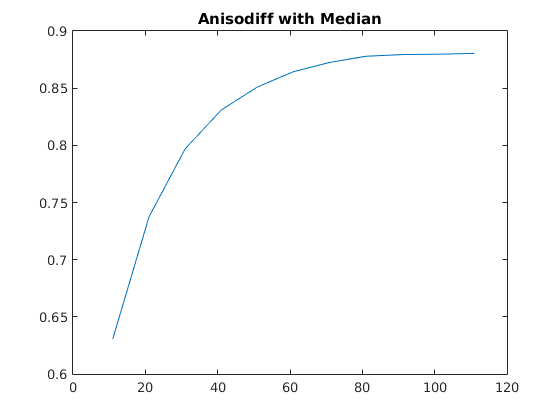
\includegraphics[width=1\textwidth]{./Figures/Results/anisodiffWithMedianJump.png}
        \caption{Con saltos}
        \label{fig:thermalforanisodiffwithmediana}
  \end{subfigure}
  \begin{subfigure}[b]{0.48\textwidth}
        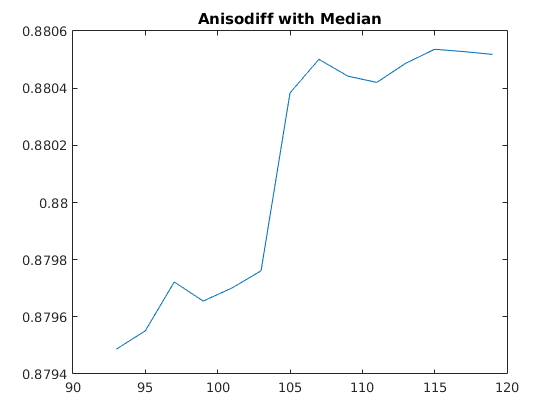
\includegraphics[width=1\textwidth]{./Figures/Results/anisodiffWithMedianCentrado.png}
        \caption{Centrado en la zona mas intensa}
        \label{fig:thermalforanisodiffwithmedianacentered}
  \end{subfigure}
  \begin{subfigure}[b]{0.48\textwidth}
        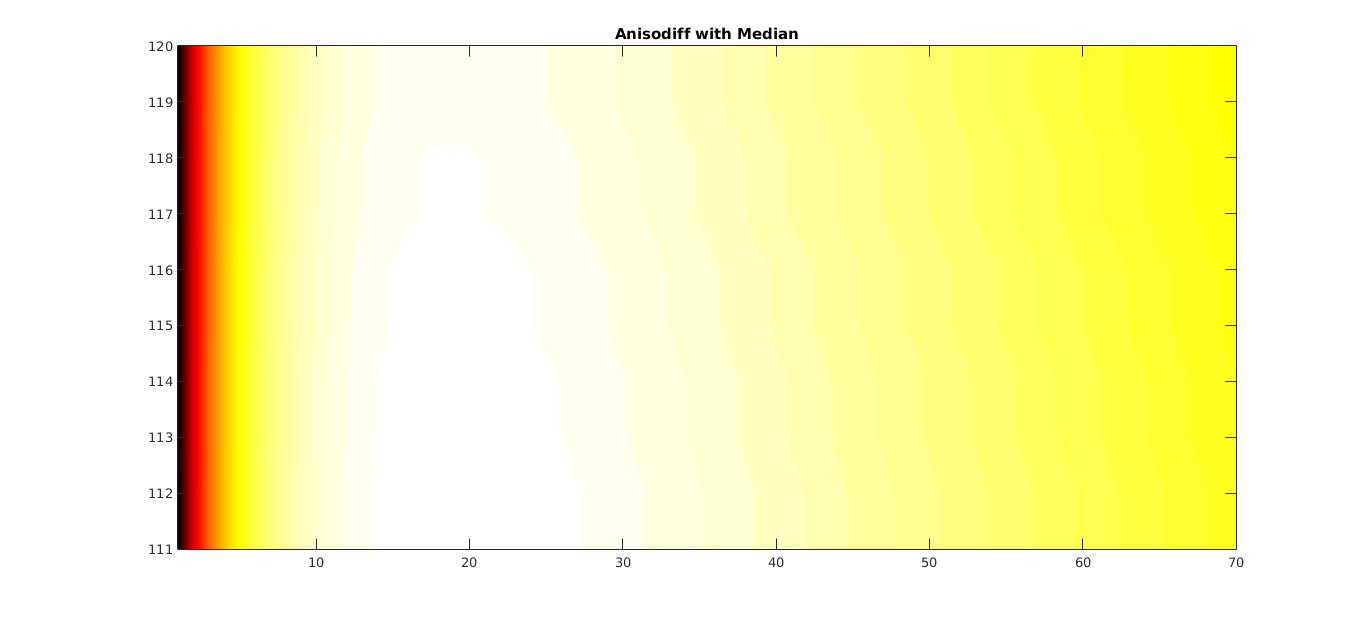
\includegraphics[height=5.3cm,width=1\textwidth]{./Figures/Results/anisodiffWithMedianColorMap.png}
        \caption{Mapa de calor}
        \label{fig:thermalforanisodiffwithmedianacentered}
  \end{subfigure}
  \begin{subfigure}[b]{0.48\textwidth}
        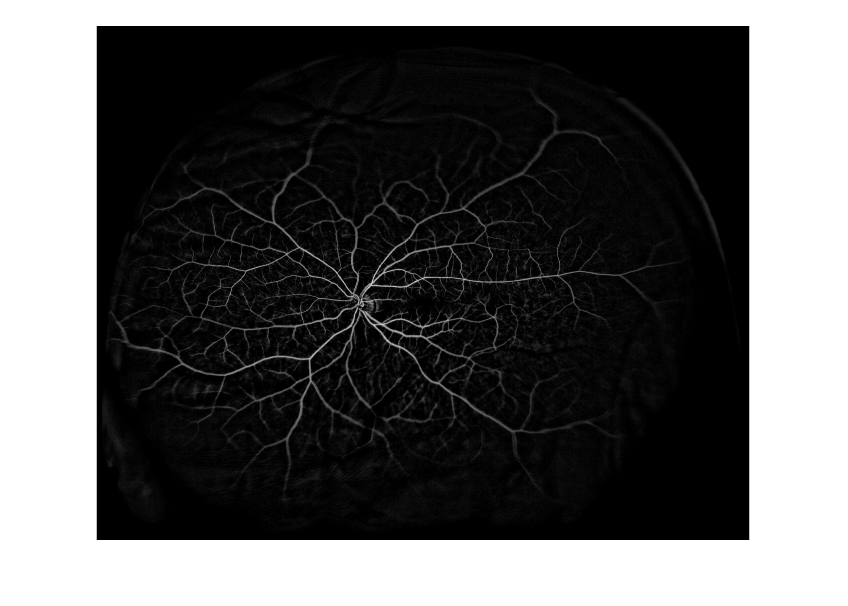
\includegraphics[width=1\textwidth]{./Figures/Results/anisodiffWithMedianV115I19A09146.png}
        \caption{Resultado con V:115 I:19 A:0.9146}
        \label{fig:thermalforanisodiffwithmedianacentered}
  \end{subfigure}
	\label{fig:thermalfigure}
	\caption{Resultado utilizando Mediana y Filtro Anisotr\'opico}
\end{figure}


\begin{figure}[H]
	\centering
	\begin{subfigure}[b]{0.48\textwidth}
        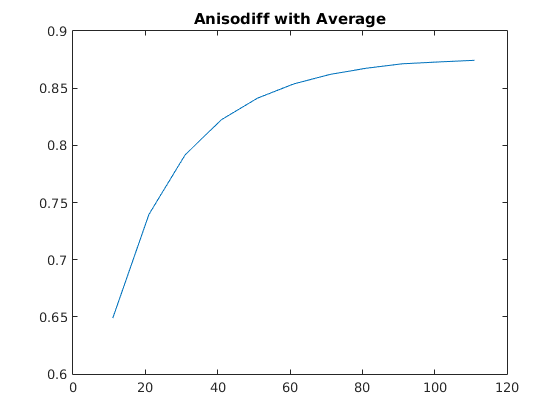
\includegraphics[width=1\textwidth]{./Figures/Results/anisodiffWithAverageJump.png}
        \caption{Con saltos}
        \label{fig:thermalforanisodiffwithmediana}
  \end{subfigure}
  \begin{subfigure}[b]{0.48\textwidth}
        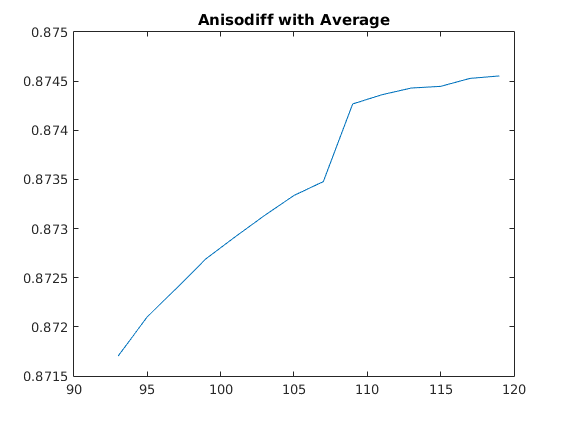
\includegraphics[width=1\textwidth]{./Figures/Results/anisodiffWithAverageCentrado.png}
        \caption{Centrado en la zona mas intensa}
        \label{fig:thermalforanisodiffwithmedianacentered}
  \end{subfigure}
  \begin{subfigure}[b]{0.48\textwidth}
        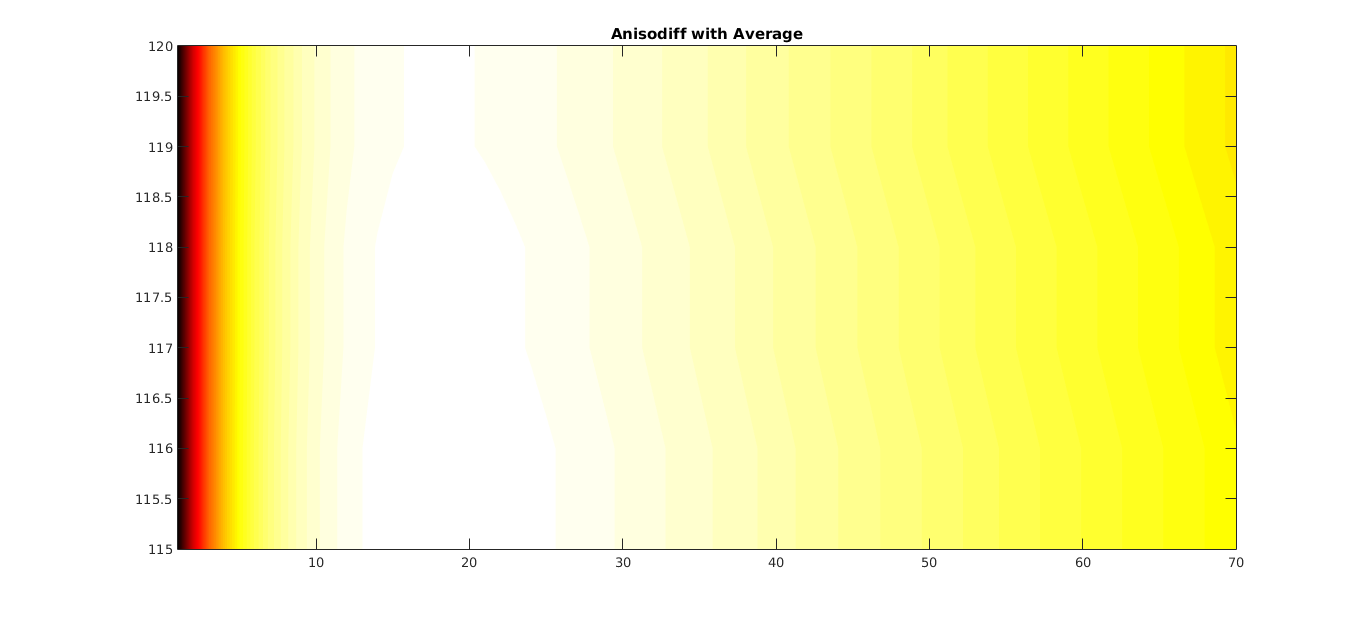
\includegraphics[height=5.3cm,width=1\textwidth]{./Figures/Results/anisodiffWithAverageColorMap.png}
        \caption{Mapa de calor}
        \label{fig:thermalforanisodiffwithmedianacentered}
  \end{subfigure}
  \begin{subfigure}[b]{0.48\textwidth}
        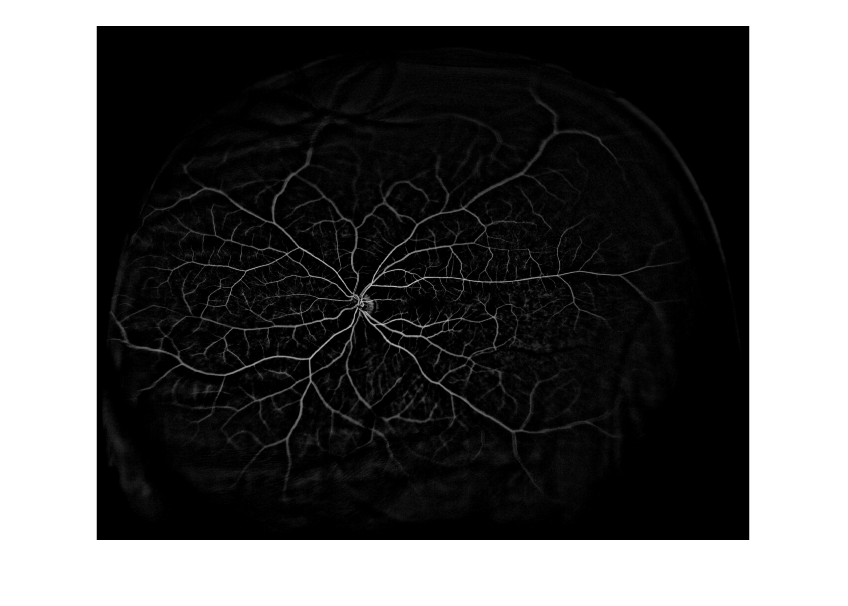
\includegraphics[width=1\textwidth]{./Figures/Results/anisodiffWithAverageV119I18A09077.png}
        \caption{Resultado con V:119 I:18 A:0.9077}
        \label{fig:thermalforanisodiffwithmedianacentered}
  \end{subfigure}
	\label{fig:thermalfigure}
	\caption{Resultado utilizando Media y Filtro Anisotr\'opico}
\end{figure}

\begin{figure}[H]
	\centering
	\begin{subfigure}[b]{0.48\textwidth}
        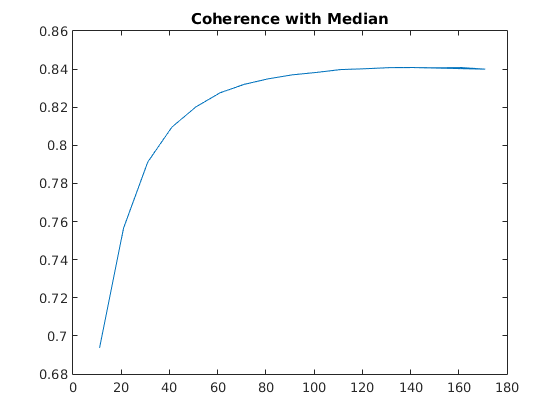
\includegraphics[width=1\textwidth]{./Figures/Results/coherenceWithMedianJump.png}
        \caption{Con saltos}
        \label{fig:thermalforanisodiffwithmediana}
  \end{subfigure}
  \begin{subfigure}[b]{0.48\textwidth}
        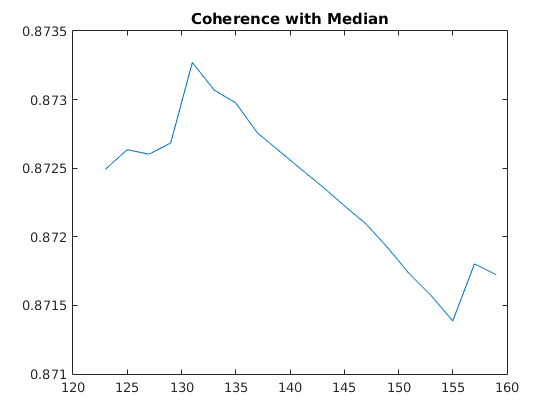
\includegraphics[width=1\textwidth]{./Figures/Results/coherenceWithMedianCentrado.png}
        \caption{Centrado en la zona mas intensa}
        \label{fig:thermalforanisodiffwithmedianacentered}
  \end{subfigure}
  \begin{subfigure}[b]{0.48\textwidth}
        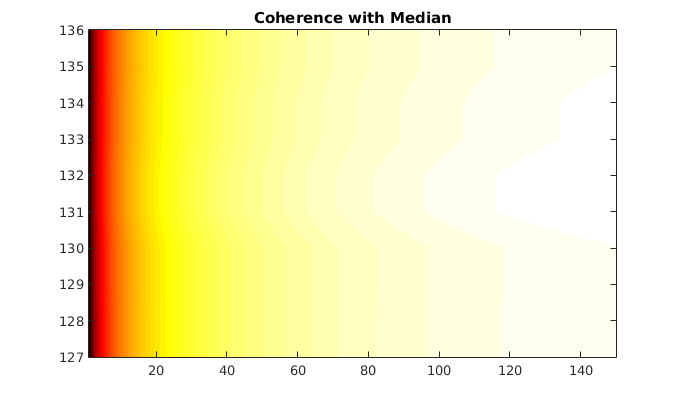
\includegraphics[height=5.3cm,width=1\textwidth]{./Figures/Results/coherenceWithMedianColorMap.png}
        \caption{Mapa de calor}
        \label{fig:thermalforanisodiffwithmedianacentered}
  \end{subfigure}
  \begin{subfigure}[b]{0.48\textwidth}
        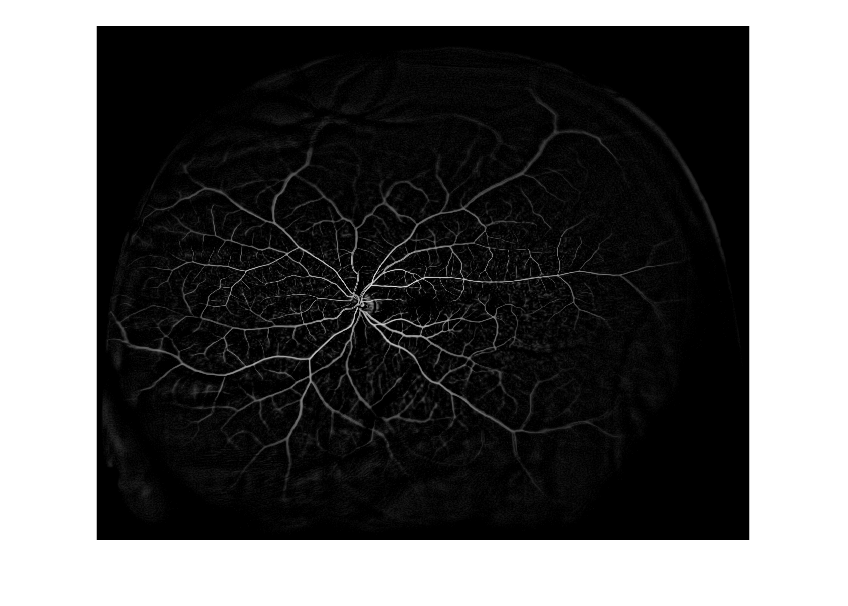
\includegraphics[width=1\textwidth]{./Figures/Results/coherenceWithMedianV131I150A09080.png}
        \caption{Resultado con V:131 I:150 A:0.9080}
        \label{fig:thermalforanisodiffwithmedianacentered}
  \end{subfigure}
	\label{fig:thermalfigure}
	\caption{Resultado utilizando Mediana y Filtro Anisotr\'opico}
\end{figure}

\begin{figure}[H]
	\centering
	\begin{subfigure}[b]{0.48\textwidth}
        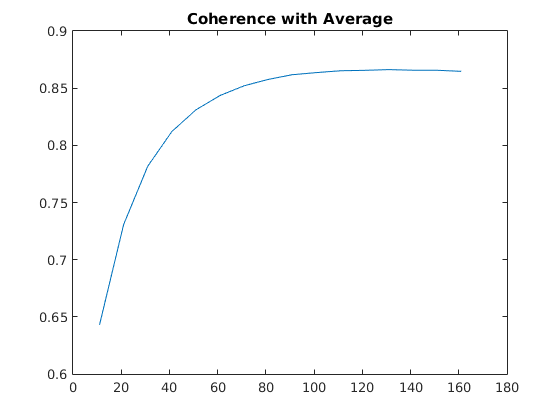
\includegraphics[width=1\textwidth]{./Figures/Results/coherenceWithAverageJump.png}
        \caption{Con saltos}
        \label{fig:thermalforanisodiffwithmediana}
  \end{subfigure}
  \begin{subfigure}[b]{0.48\textwidth}
        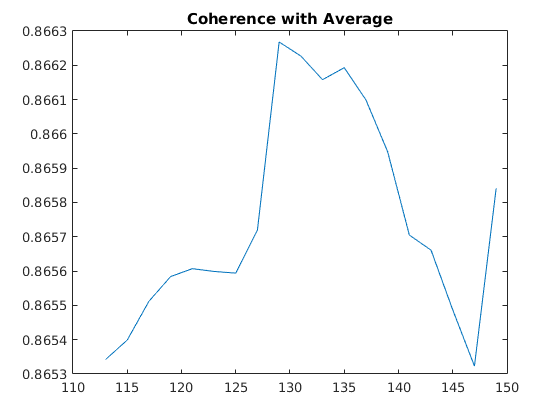
\includegraphics[width=1\textwidth]{./Figures/Results/coherenceWithAverageCentrado.png}
        \caption{Centrado en la zona mas intensa}
        \label{fig:thermalforanisodiffwithmedianacentered}
  \end{subfigure}
  \begin{subfigure}[b]{0.48\textwidth}
        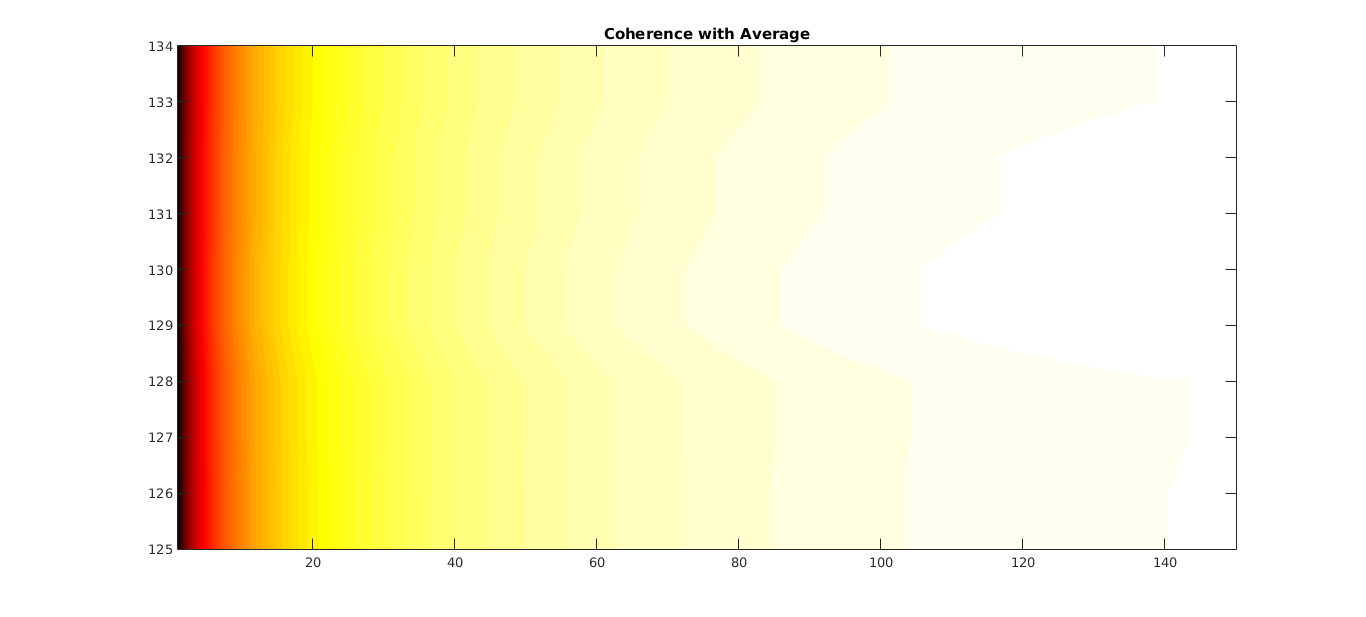
\includegraphics[height=5.3cm,width=1\textwidth]{./Figures/Results/coherenceWithAverageColorMap.png}
        \caption{Mapa de calor}
        \label{fig:thermalforanisodiffwithmedianacentered}
  \end{subfigure}
  \begin{subfigure}[b]{0.48\textwidth}
        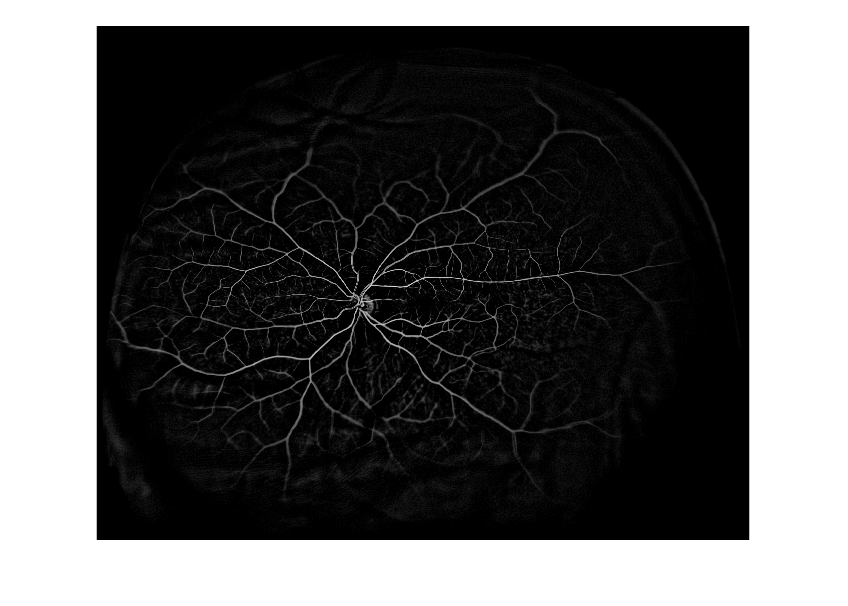
\includegraphics[width=1\textwidth]{./Figures/Results/coherenceWithAverageV129I150.png}
        \caption{Resultado con V:129 I:150 A:0.8990}
        \label{fig:thermalforanisodiffwithmedianacentered}
  \end{subfigure}
	\label{fig:thermalfigure}
	\caption{Resultado utilizando Mediana y Filtro Anisotr\'opico}
\end{figure}

%\begin{figure}[H]
%\centering
%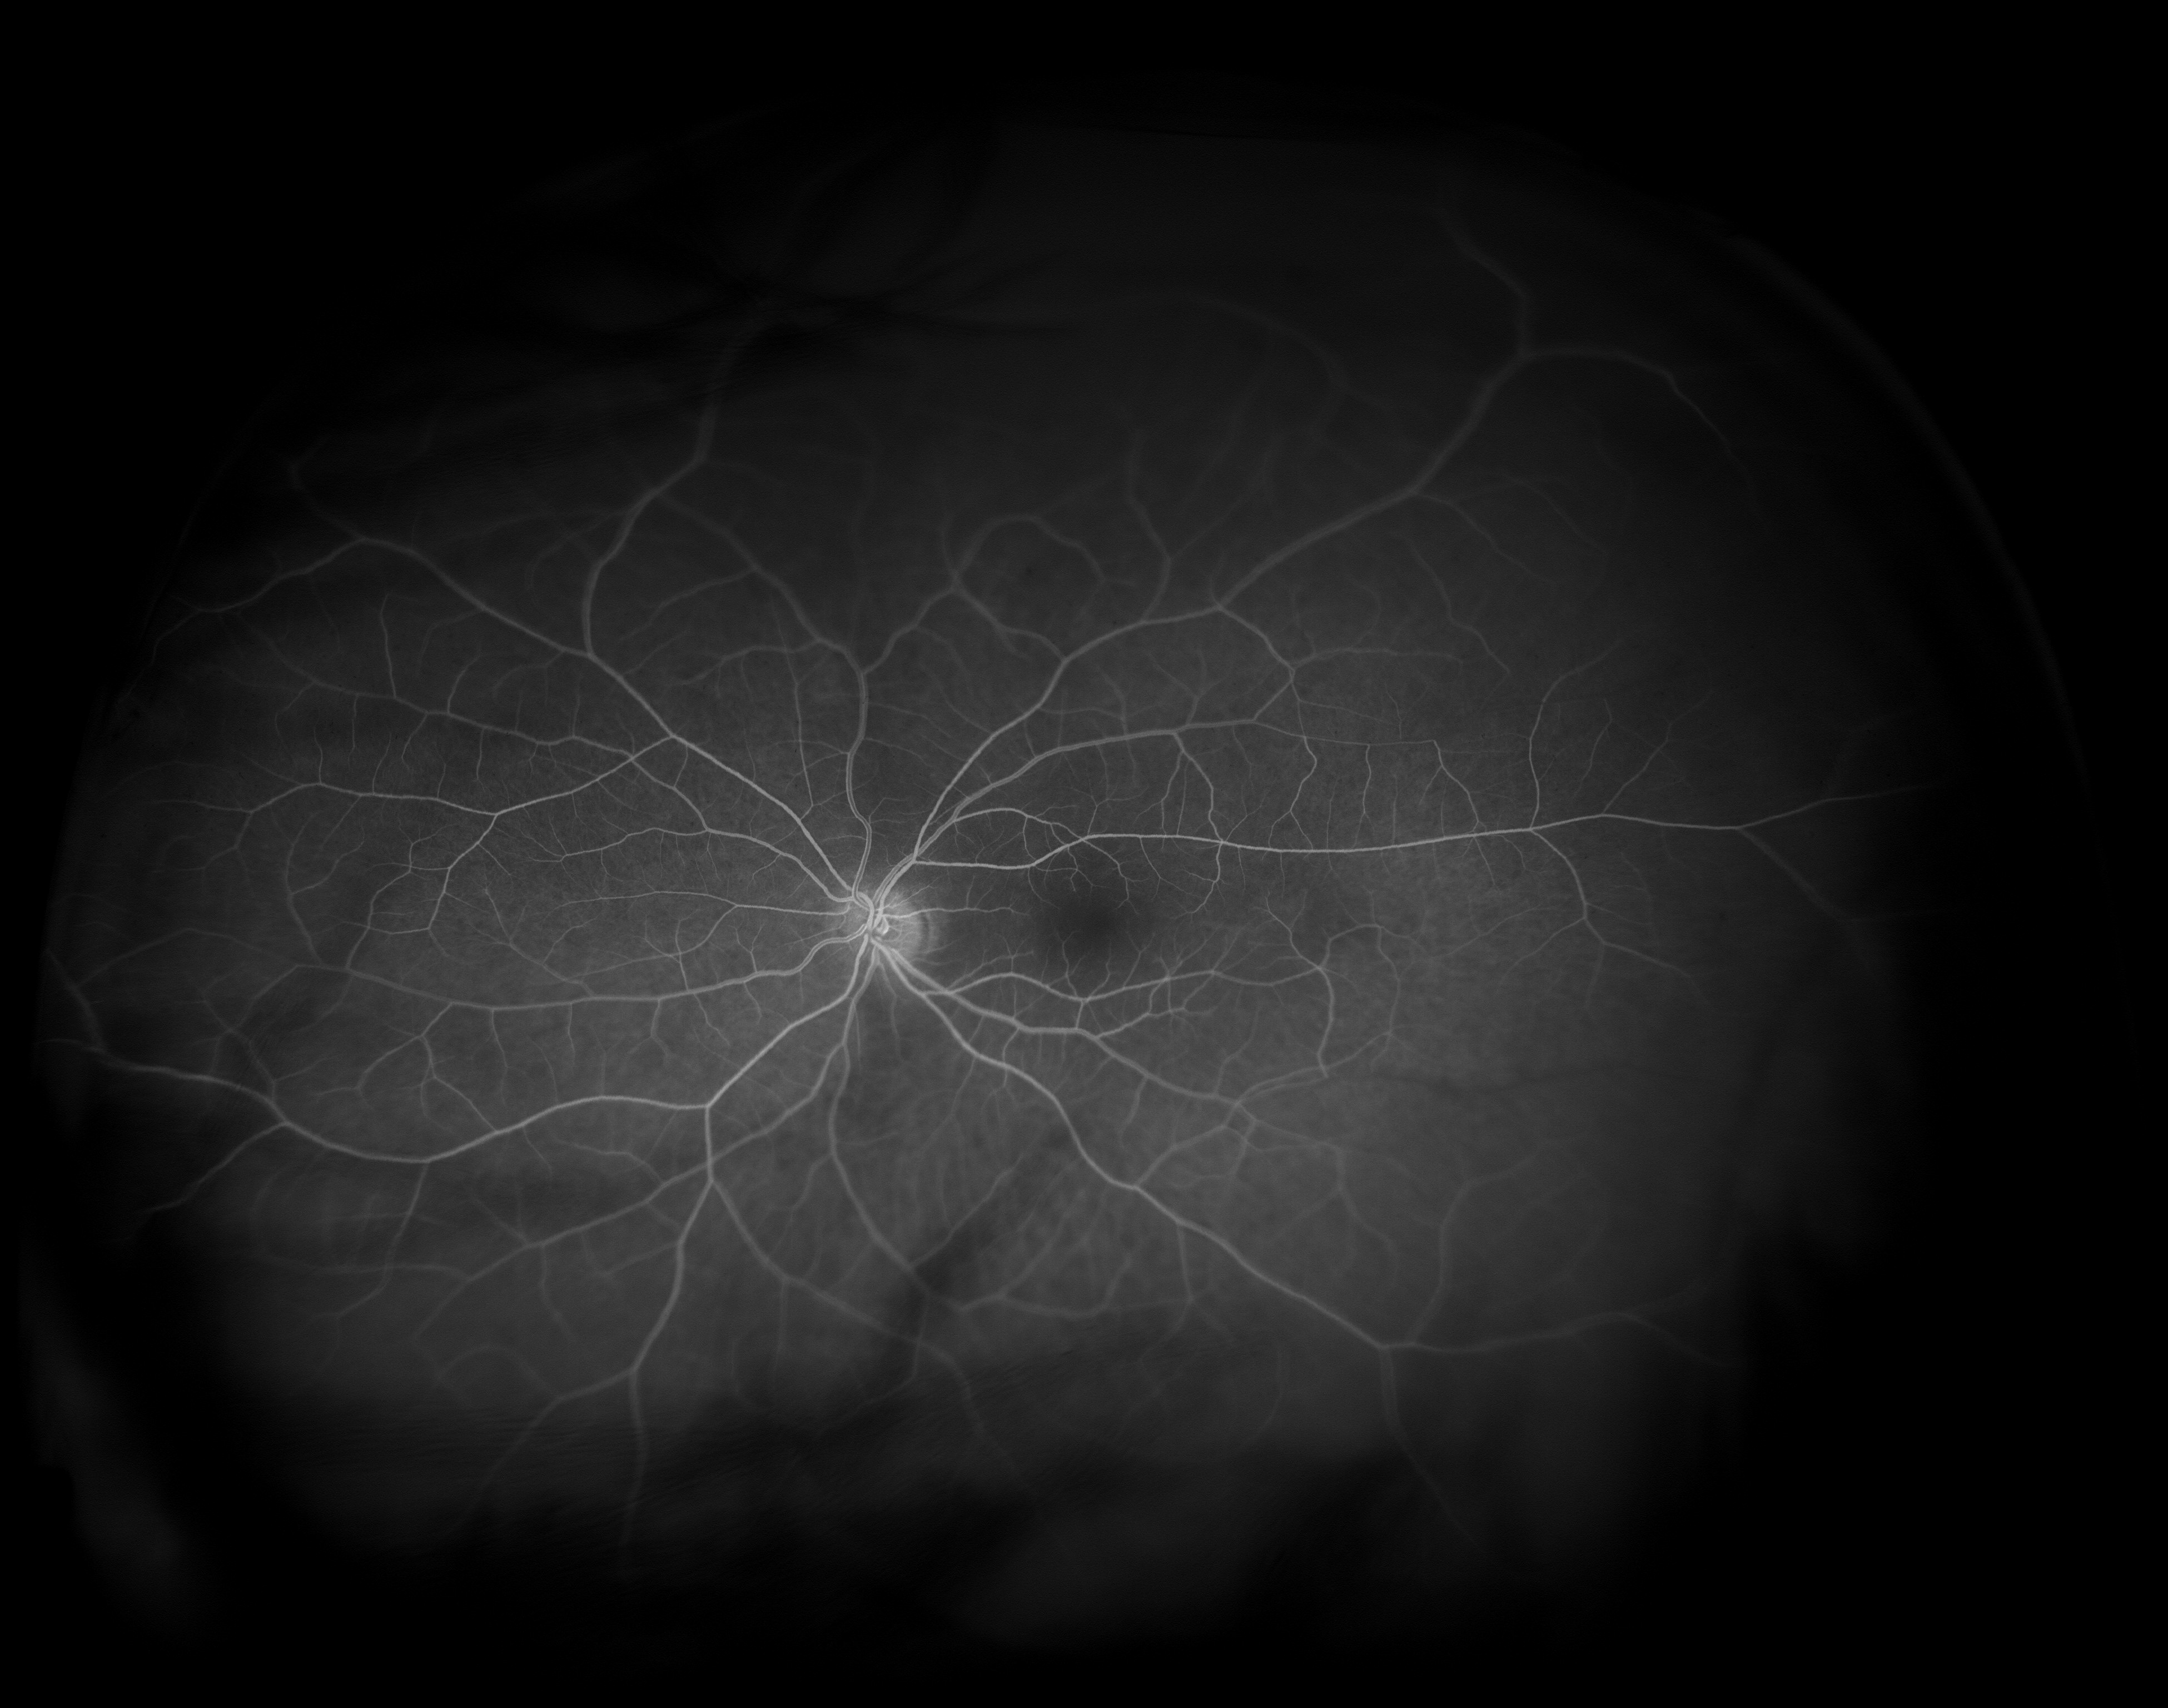
\includegraphics[width=0.9\textwidth]{./Figures/Results/GER2.png}
%\label{fig:lightfilter}
%\caption{Imagen de referencia}
%\end{figure}

%Dada la naturaleza de los experimentos decidimos que la mejor manera de mostrar los resultados era un mapa de %calor(Figura \ref{fig:thermalforanisodiffwithmediana}) y para poder visualizar mejor el comportameniento en la zona %de calor mas intenso aislamos la regi\'on (Figura \ref{fig:thermalforanisodiffwithmedianacentered}) y lo graficamos %en tres dimensiones (Figura \ref{fig:centeredregionthermal}).

%\begin{figure}[H]
%	\centering
 % 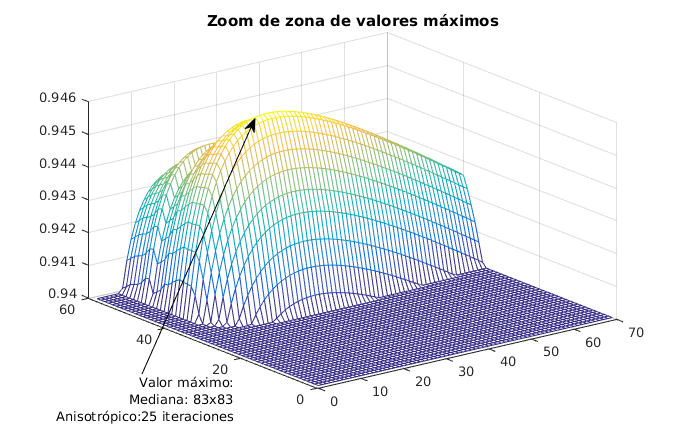
\includegraphics[width=0.75\textwidth]{./Figures/FiguraEvaluacionMaximosAnisodiff.png}
  %\caption{Regi\'on \'optima graficada en tres dimensiones}
  %\label{fig:centeredregionthermal}
%\end{figure}


%FALTAN EXPERIMENTOS:
\begin{description}
  \item[Media con anisodiff] En algun momento descartamos la media pero no tenemos datos guardados para mostrar
  \item[Media con coherencia] En algun momento descartamos la media pero no tenemos datos guardados para mostrar
  \item[Mediana con coherencia] Hicimos el de difusion anistropica, y el de coherencia pudimos buscarle la vuelta ahora para hacerlo mas rapido
\end{description}

\subsection{Comparativa}

Pendiente de los resultados de los experimentos.












